\chapter{Project Development} \label{chap:implementation}

All the theory explained in Chapter \ref{chap:theory} and the details of the study case presented in Chapter \ref{chap:robi} lead us to the definition of the requirements for the implementation of the motor driver needed by the ROBI' project. This driver, defined as the \ac{WMU} in Chapter \ref{chap:robi}, should be able to apply both driving techniques, trapezoidal and sinusoidal, and to execute different motor control methods for the \ac{PMSM} in-wheel motors. The driving and control methods should be selected by future developers, depending on the application and on the algorithm needed for the control of the overal displacement of ROBI'.

This chapter is divided into three sections: the first section contains a description of the hardware implementation of the driver; the second section explains the implementation of the driving techniques and control methods through embedded software; the last section describes the setup mounted to test the driving capabilities of the \ac{WMU} developed.

\section{Hardware}

The \ac{WMU}'s electronic circuit is based on an open architecture proposed by \acf{TI} to be implemented together with the use of their \ac{IC} \ac{MOSFET} inverter driver DRV8302. This architecture was implemented in a project developed by the Swedish engineer Benjamin Vedder called VESC, which consists in the design of an \acf{ESC}, its \ac{PCB} layout design and the implementation of the source code used to drive a \ac{BLDC} motor (\citeauthor{VedderVesc}, \citeyear{VedderVesc}). The hardware design of the VESC board was not modified for this thesis in order to identify, after the implementation and the testing of the motor control algorithms, what could be changed to obtain a better performance from the in-wheel motors mounted on ROBI'.

\subsection{VESC Board}

The VESC board was conceived and designed to be used as an \ac{ESC} in electric skateboards with the intention to create one of the best \ac{ESC}s available. Since it was planned to be used in a skateboard, it has a small form-factor and it can be used for different applications with similar power demand. The hardware can also be modified by changing specific components to drive motors with higher power demand or by modifying the \ac{PCB} layout design following the schematic design. The original schematic files can be found attached in Appendix \ref{appendix:vesc_schematics} for reference.

\begin{figure}[htbp]
\centering
\includegraphics[width=10cm]{Images/pcb_front.png} 
\caption[VESC Front Side]{Front Side of the VESC Board. The three wires at soldered at the right edge of the board are connected to the three phases of the brushless motor.}
\label{fig:pcb_front}
\end{figure}

The \ac{PCB} provided as part of the VESC project is a four-layer, $40mm \times 60mm$, FR-4 board, with pads for components on the both external layers. The use of both external layers to place components and the four layers to interconnect the circuits allows the board to keep a small form factor.

The board different functional components of the board and their considerations regarding the implementation of the \ac{WMU} will be explained in this section.

\subsection{Power Supply Input}
The power is supplied into the board by means 2 wires soldered into large pads placed close to the three-phase inverter nodes $V\_SUPPLY$ and $GND$. $V\_SUPPLY$ and $GND$ are the positive and negative nodes of the power supply source respectively. The power is supplied from a power regulator for static applications or from a battery for mobile applications, like in the case of ROBI'. It is also specified in the schematics that there should be a bulk capacitor connected in parallel to the power supply port.

\begin{figure}[htbp]
\centering
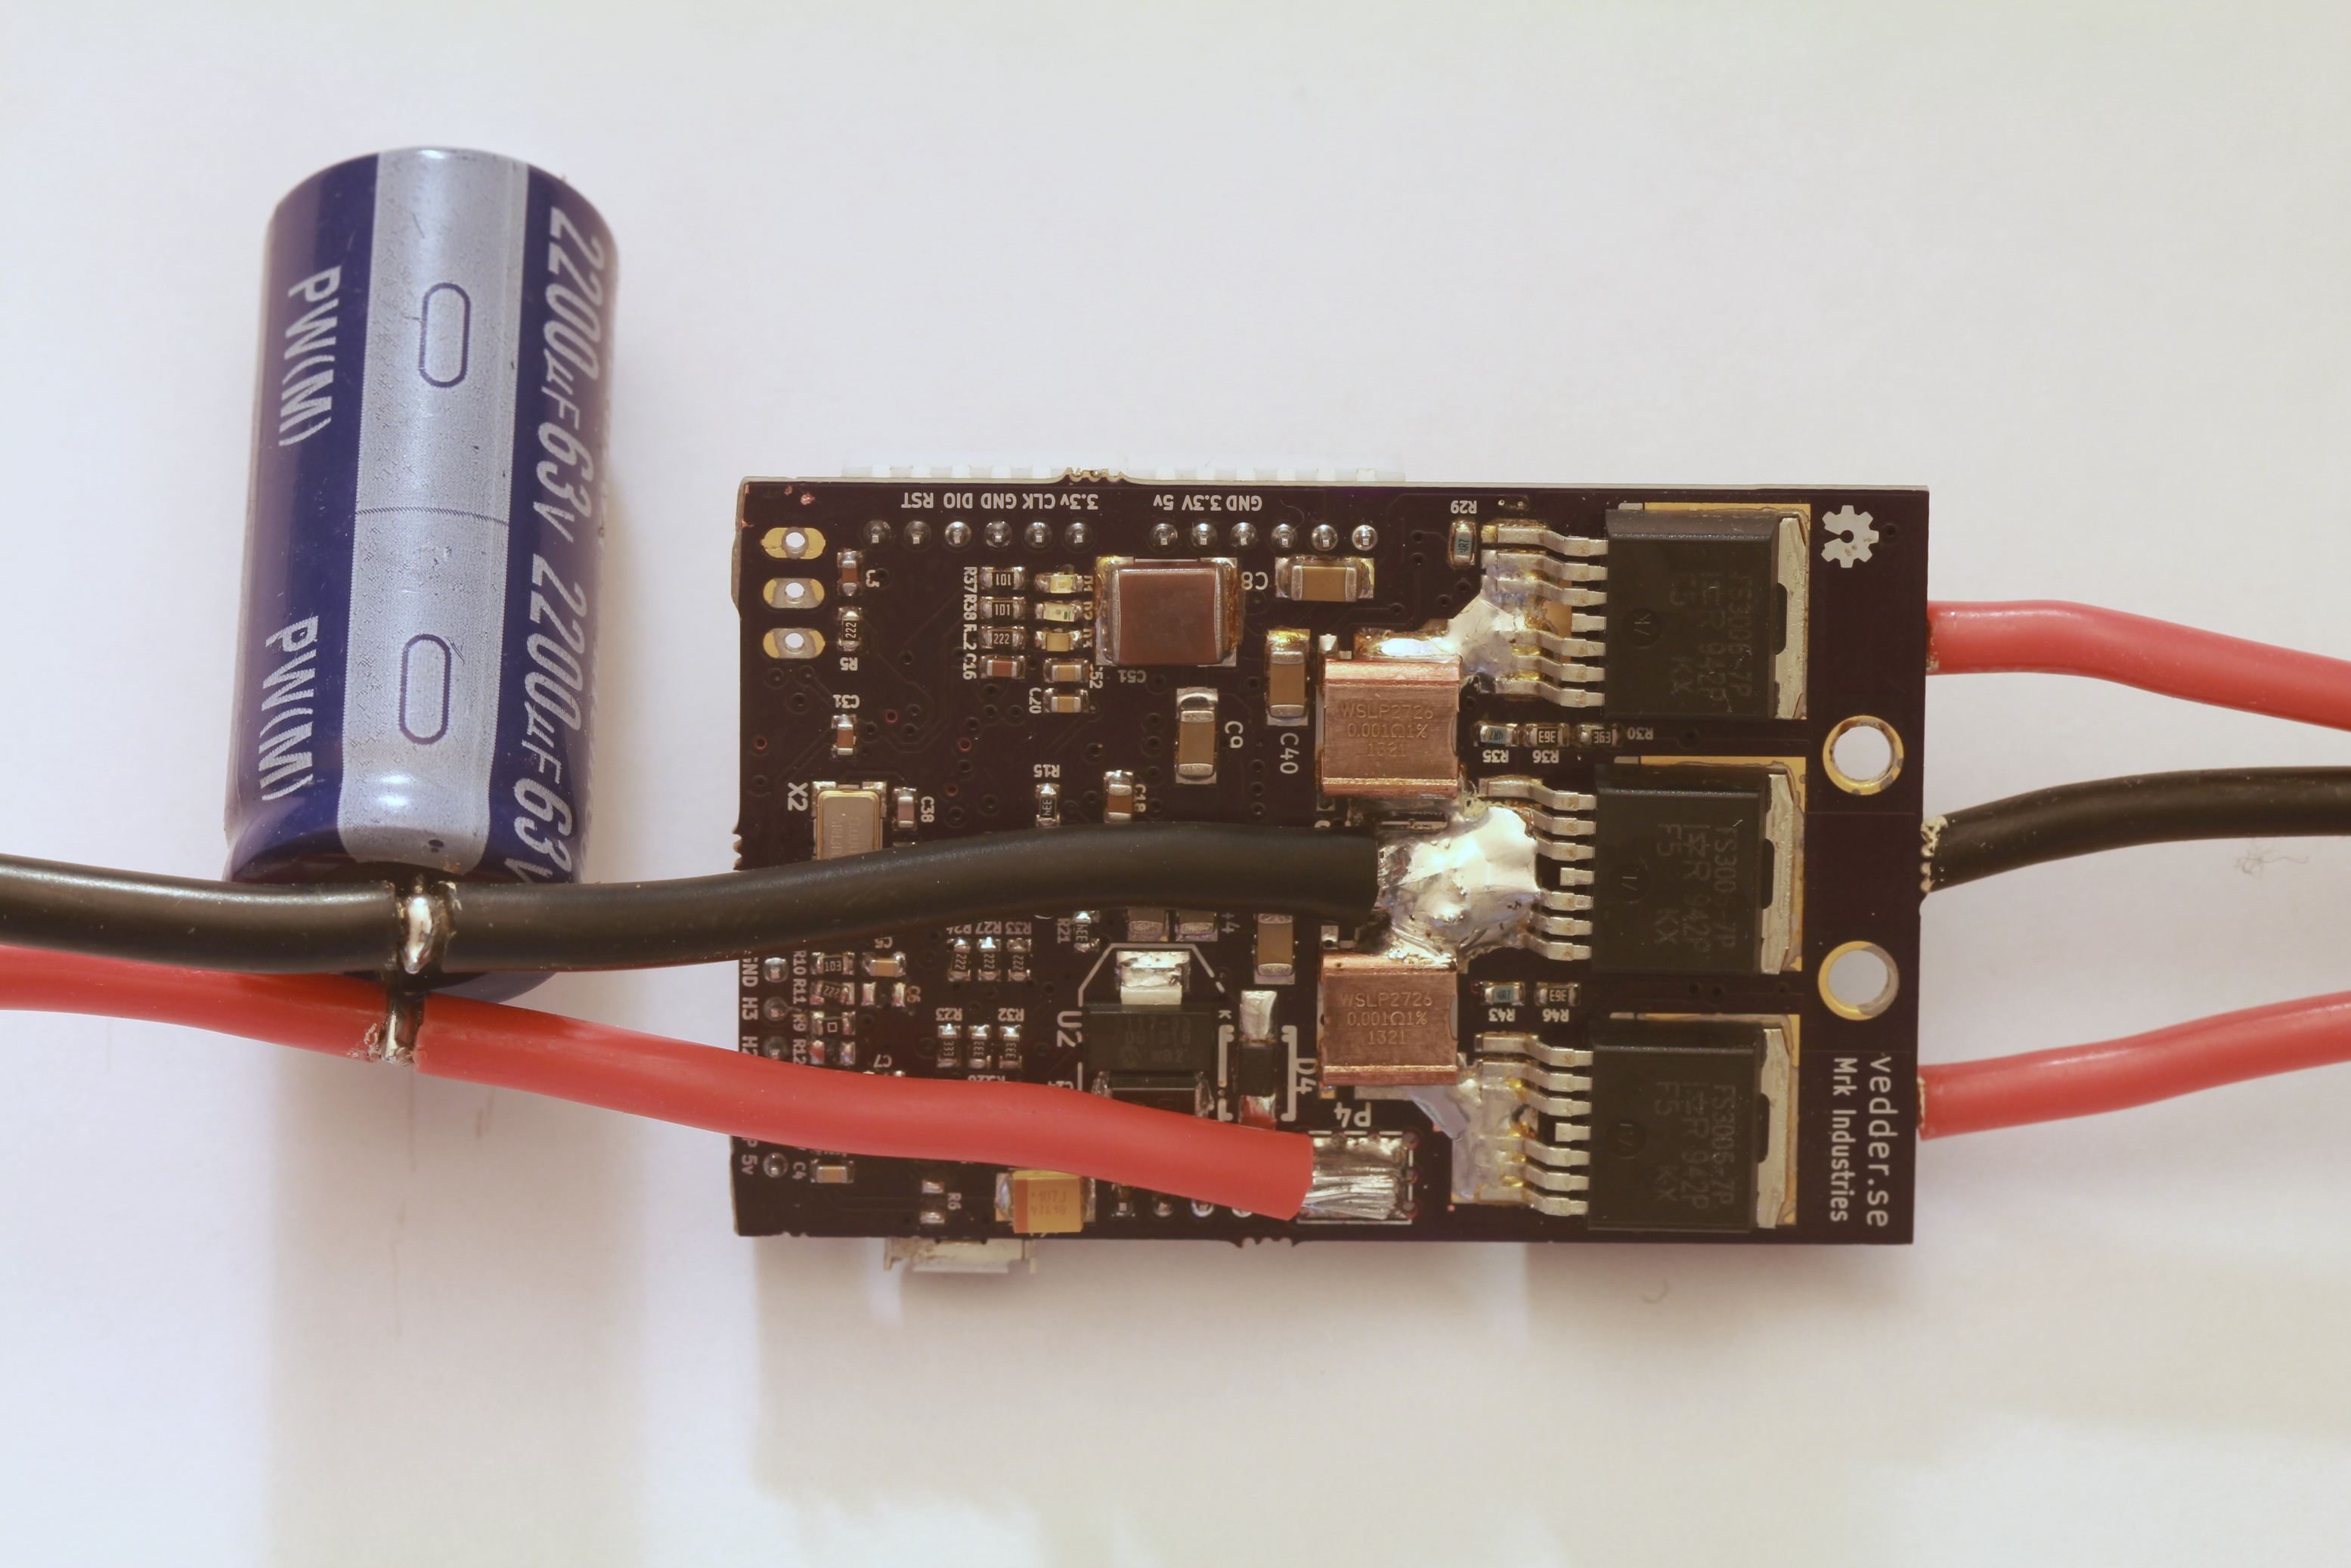
\includegraphics[width=10cm]{Images/pcb_back.png} 
\caption[VESC Back Side]{Back Side of the VESC board. The red and black wires are the power supply input $V\_SUPPLY$ and $GND$ respectively.}
\label{fig:pcb_back}
\end{figure}

\subsubsection{Power Supply Range}

The voltage range of the VESC board is defined by the \ac{MOSFET} driver \ac{IC} $DRV8302$, which specifies an operating supply voltage range from $8V$ to $60V$, but allows a maximum voltage supply up to $65V$ \ref{DRV8302}. All the other components of the board, mainly capacitors and power \ac{MOSFET}s, must be selected according to this voltage range.

The current range of the board is limited by the \ac{MOSFET}s current limit and by the width of the traces in the \ac{PCB}. These maximum values will be addressed later in the section dedicated to the \ac{MOSFET} inverter used in the board.

\begin{table}[]
\centering
\caption{VESC Board Operating Ranges}
\label{table:vesc_ranges}
\begin{tabular}{@{}lll@{}}
\toprule
Input voltage          	& $8$ to $60V$ 	\\
Maximum output current 		   	& $50A$		\\
Peak output current     & $240A$ 		\\
\bottomrule
\end{tabular}
\end{table}

\subsubsection{Bulk Electrolytic Capacitor}

It is important to place a bulk capacitance with an appropiate capacitance value and voltage range in parallel to the input of the power supply of a motor drive system. The main objective of a bulk capacitance is to control the voltage deviation at the input of a system when the converter is responding to an output load transient, meaning that if there is a load increase and the power supply is not able to provide the current instantaneously for the motor, the current must be provided by the bulk capacitor. The higher the capacitance at the input of the system, the lower the deviation at the load, but this comes at a cost of price and space, since the capacitance value of a capacitor is proportional to the size of its parallel plates. The value of the input bulk capacitor is determined mainly by the following factors:

\begin {enumerate}
	\item The largest amount of current required by the motor
	\item The capacitance of the power supply and its ability to source current
	\item The parasitic inductance between the power supply and the motor
	\item The acceptable voltage ripple
	\item The type of motor
\end {enumerate}

The datasheet of a motor driver should generally provide a recommended value for the bulk capacitor, but it is necessary to calculate and test the value to determine if it's appropiate. The voltage rating of a bulk capacitor must be higher than the value of the power supply to provide a margin for cases in which the motor transfers energy to the supply, which would increase its voltage and would damage a capacitor with a smaller value than the resulting voltage. We can calculate the capacitance value by using the following formula (\citeauthor{bulkCap}, \citeyear{bulkCap}):

\begin{equation} \label{current_ripple_2}
	C = \frac{1.21 \cdot I_{tr}^{2} \cdot L}{\Delta V^{2}}
\end{equation}

Since there is no filtering inductance in the system, we can consider a stray inductance of $50 nH$ in the calculation. If we consider a transient current $I_{tr}$ equal to the rated current of the in-wheel motor, $14 A$ approximatedly, and a voltage ripple of $100 mV$, we obtain a capacitance value of $1185.8\mu F$ for the bulk capacitance. Looking for available capacitor values, we increased the value of the capacitor to $2200\mu F$ and, considering the maximum input voltage value of the motors, the common practice is to double that value, so we defined a voltage range of $75V$, which is a typical value for a commercially available capacitor.

It is important to note that since the value of this capacitance is large, also its size will be large, therefore it's important to consider its dimensions to setup a mechanically stable position for such capacitance with aims of avoiding hardware malfunction.

\subsubsection{Power Supply Wiring}

The strategy of soldering the wires directly to the pads in the \ac{PCB} helps reduce the size and cost of the board since it avoids the use of large power traces in that would be needed if a regular receptacle connector was to be used.

Anyway, the practice of soldering a wire directly to a \ac{PCB} is discouraged mainly in circuits that will be mounted in a system designed to be in movement (i.e. automotive or aerospace applications) because the wire used in these applications is made of delicate copper strands which can break easily with movement of the board or of the wires and cause a short circuit or a loose contact, both of which might lead to catastrophic failures , so there is a risk in this board since it will be mounted in systems that will be in constant movement (\citeauthor{connectors}, \citeyear{connectors}). Since this board was designed this way to reduce space consumption, the trade-off between safety and size was balanced into the size constraints, therefore some cautions must be taken to avoid problems, mainly because these wires carry a considerable amount of current and they pass over many components of the board as seen in Figure \ref{fig:pcb_back}.

The first consideration to be made is the wire gauge and insulation type. The wire gauge is a measurement of the wire diameter, which determines the amount of electric current that a wire can safely carry, as well as its electrical resistance and weight. For this board, it is suggested to use short wires to avoid a large voltage drop and to ease the handling of such wire until it reaches the output of the enclosure that will protect the circuit.

The second consideration regarding the wire selection is the insulation material. Since the current passing through the copper also implies power consumption due to the resistance of the copper, there is heat transfer from the wire to its surroundings. To protect the copper strands from its surroundings and vice versa, wires are covered by an insulating material, which has low thermal and electrical conductivity.

Since the heat exchange calculation of the wire would require many assumptions, it’s a normal practice to select the type of wire using tables that consider the temperature rise in the wire according to different currents and lengths. In the case of the \ac{PMSM} motor used in ROBI', the maximum rated current would be approximately $14A$, which would lead us to select a wire with a diameter between $2.1mm$ and $2.6mm$, based on Table \ref{table:awg}. This selection would depend on the number of cores from which the wire is constructed: the bigger the ammount of cores, the more flexible the wire is, but also the diameter becomes larger.

\begin{table}[]
\centering
\caption{American Wire Gauge current load ratings in function of the number of cores of the wire (\citeauthor{awg}, \citeyear{awg})}
\label{table:awg}
\begin{tabular}{@{}llllllll@{}}
\toprule
\multirow{2}{*}{AWG} & \multirow{2}{*}{D {[}mm{]}} & \multicolumn{6}{l}{Maximum Current Load Ratings {[}A{]}}                         \\
                     &                                    & 1  & 2 - 3 & 4 - 6 & 7 - 24 & 25 - 42 & > 43  \\
\midrule
16                   & 1.3                                & 15     & 10          & 8           & 7            & 6             & 5            \\
14                   & 1.6                                & 24     & 15          & 12          & 10           & 9             & 7.5          \\
12                   & 2.1                                & 34     & 20          & 16          & 14           & 12            & 10           \\
10                   & 2.6                                & 52     & 30          & 24          & 21           & 18            & 15           \\
\bottomrule
\end{tabular}
\end{table}

\subsection{Power MOSFET Three-Phase Inverter}

The three-phase inverter used in the VESC board is based on the power \ac{MOSFET} IRFS7530-7PPbF, manufactured by the semiconductor company International Rectifier. The schematic design of the inverter can be seen in Figure \ref{fig:sch2} in Appendix \ref{appendix:vesc_schematics}. The \ac{PMAC} motor is connected to the board by soldering its phase terminals directly to the node pads in the middle of each branch of the inverter, which is located at the bottom edge of the board, as seen in Figure \ref{fig:pcb_front}.

\begin{table}[]
\centering
\caption{IRFS7530-7PPbF Absolute Maximum Rating}
\label{table:irf_ranges}
\begin{tabular}{@{}ll@{}}
\toprule
Continuous drain current & $240A$ \\
Maximum power dissipation (\@25\degree)	& $375W$ \\
Linear derating factor & $2.5W/\degree C$ \\
Drain-to-Source breakdown voltage & $60V$ \\
Drain-to-Source on-resistance & $1.5m\Omega$ \\
\bottomrule
\end{tabular}
\end{table}

This \ac{MOSFET} is based on the HEXFET Power \ac{MOSFET} technology, which is a Vertical Double-diffused MOS transistor (VDMOS) with hexagonal elementary cells in parallel which maximizes the $W/L$ ratio of the transistor, providing a low on-resistance value $R_{DS(ON)}$ (\citeauthor{GhioniPowerElec}, \citeyear{GhioniPowerElec}).

We can see from Table \ref{table:irf_ranges} that the maximum power dissipation of the \ac{MOSFET} is lower than the rated power of the in-wheel motors mounted on ROBI', therefore, the maximum rated values of the motor won't be reached using this model of transistors. It is also important to note that the maximum power dissipation implies a junction temperature of $25\degree C$, which means that the heat of the \ac{MOSFET} package should be dissipated by a heat sink, which is not implemented nor considered in the VESC board. If the heat is not dissipated from the transistors, the power decreases following the linear derating factor.

\subsubsection{Switching Times}\label{switching_times}

As mentioned in \ref{subsection:inverter}, power \ac{MOSFET}s have large parasitic capacitances that need to be charged in order to allow the activation of the transistor. This behaviour also affects the switching time, which is the time that a transistor takes to turn on and turn off completely.

The switching time of a transistor is therefore defined by the capability of the driving circuit to provide current to charge the parasitic capacitances in the gate and to draw current from them.

To determine the switching time of a \ac{MOSFET} is necessary to analyse the driving circuit and the parasitic capacitances of the transistor. The information regarding the switching time of the transistor is normally available in the device datasheet.

\begin{table}[]
\centering
\caption{IRFS7530-7PPbF Dynamic Electrical Characteristics}
\label{table:switchtime}
\begin{tabular}{@{}ll@{}}
\toprule
Total gate charge 		& 236 nC \\
Gate-to-Source charge 	& 62 nC \\
Gate-to-Drain charge 	& 73 nC \\
Turn-On delay time   	& 24 ns \\
Rise time       		& 102 ns \\
Turn-Off delay time     & 168 ns \\ 
Fall time               & 79 ns \\
Input capacitance  		& 12.9 nF \\
\bottomrule
\end{tabular}
\end{table}

It is important to notice also the conditions on which the electrical characteristics of the device where obtained. In this case, it is stated in the datasheet that the transistor had a gate resistance $R_{G}$ of $2.7\Omega$, a gate-source voltage $V_{GS}$ of $10V$, a $V_{DC}$ equal to $30V$ and the current flowing through the device was $100A$.

In the case of the IRFS7530-7PPbF, we can calculate that the minimum period of time to turn on and turn off the transistor is $373 ns$, which is equal to the sum of the turn-on delay time, rise time, turn-off delay time and fall time (Table \ref{table:switchtime}). The inverse of the minimum switching period defines the maximum switching frequency of the transistor $f_{switch,max}$ which is equal to $2.68 MHz$. Since the time constant $\tau = L/R$ of the motor is equal to $4.75 ms$, which is much larger than $373 ns$, we can see that the switching frequency of the IRFS7530-7PPbF doesn't represent a limitation for implementing the driving methods explained previously. This switching frequency limitation should be considered instead at the moment of the implementation of the \ac{PWM} signal generation.

If we look at the \ac{MOSFET}s on the inverter in the VESC board, we can see that there is a $4.7\Omega$ resistance connected between the driver and the gate, which might change the driving current of the device. We must also keep an eye on the $V_{GS}$ value applied by the \ac{MOSFET} driver not to be lower than $10V$.

\subsection{MOSFET Driver}

The central component in the VESC board, around which the rest of the circuit was designed, is the \ac{IC} $DRV8302$, a brushless motor inverter driver manufactured by \ac{TI}. The complete functional block diagram can be found in Appendix \ref{appendix:drv8302_diag}.

\begin{figure}[htbp]
\centering
\includegraphics[width=10cm]{Images/drv_simple.png} 
\caption[DRV8302 Simplified Schematic]{DRV8302 Simplified Schematic}
\label{fig:drvsimple}
\end{figure}

The $DRV8302$ provides three half bridge drivers capable of driving two N-channel MOSFETs each, which solves the need to implement a high-side and a low-side circuitry to turn on each one of the transistors on the inverter, as mentioned in \ref{subsection:inverter}. For this mean, the device provides up to $30 mA$ at an output voltage $V_{GS}$ between $9.5V$ and $11.5V$ to drive the transistors, using a bootstrap gate driver architecture with trickle charge circuitry to support a duty cycle of 100\%.	

\subsubsection{Operating Range}

The $DRV8302$ can operate from a single power supply with a wide range from $8V$ to $60V$. This voltage range limits both the minimum operating voltage and the maximum operating voltage of the VESC board. The minimum operating voltage shouldn't be a problem in applications like ROBI', where the power is supplied by battery packs with a voltage larger than 12V, but if $V_{DC}$ is smaller than $8V$, the driver won't operate correctly. 

It is important to point out that the $DRV8302$ also includes an integrated switching mode buck converter with adjustable output and switching frequency, which can provide up to $1.5 A$. In the case of the VESC board, the logic level voltage $V_{DD}$ is $3.3V$, which is obtained by regulating $5V$ with a \acf{LDO} regulator. The $5V$ are obtained from the integrated buck converter of the $DRV8302$. Due to this, having a large voltage drop on the power supply, which can be caused by a big current transient, might lead to a malfunction of the motor drive system since the power supply of the microcontroller could be interrupted. This is one of the reasons why the bulk capacitance at the input of the power supply is important.

The other problem that might arise is on the other side of the voltage supply range of the device, which is $60V$. As mentioned at the end of \ref{physical_principles}, it is possible that the motor behaves as a power supply if there is a speed imposed on its rotor. Also, we explained in \ref{subsection:trapdrive} that is possible to brake the motor if we direct the current into the power supply. These behaviours lead to the posibility of a voltage increase in the motor terminals equal to the double of the voltage value of the power supply, due to the energy stored in the windings when the motor starts to brake. In the case of ROBI', this voltage might reach up to $72V$, which can lead to failure of the $DRV8302$, so we must be careful of this when braking or we must install an electronic circuit which protects the device.

\subsubsection{Switching Frequency}\label{subsec:sw_freq}

It is stated in the datasheet of the $DRV8302$ that the maximum switching frequency that can be achieved on the \ac{MOSFET} inverter by using this driver is $200 kHz$, which depends on a gate charge equal to $25 nC$. Since the gate charge of the \ac{MOSFET}s used in the inverter is much larger, we need to calculate the minimum switching period in order to be sure that this value is the same for our case. The minimum switching period is obtained from the following Equations, using the data from the dynamic electrical characteristics of the transistor (Table \ref{table:switchtime}) and the gate charge curve of the transistor (Figure\ref{fig:gatecharge}) (\citeauthor{GhioniPowerElec}, \citeyear{GhioniPowerElec}):

\begin{equation}
	t_{d(ON)} = \frac{Q_{GS}}{I_{G}} = 2.07\mu s
\end{equation}

\begin{equation}
	t_{rise} = \frac{Q_{p}}{I_{G}} = 2.433\mu s
\end{equation}

\begin{equation}
	t_{fall} = \frac{Q_{p}}{I_{G}} = \frac{Q_{p} \cdot R_{G}}{V_{GS,p}} = 97ns
\end{equation}

\begin{equation}
	t_{d(OFF)} = R_{G} \cdot C_{iss(MAX)} \ln (\frac{V_{GS,MAX}}{V_{GS,p}}) = 144.3ns
\end{equation}

\noindent
where $Q_{p}$ is the plateau charge in Figure \ref{fig:gatecharge}, equal to the Gate-to-Drain charge charge, specified in Table \ref{table:switchtime}; $I_{G}$ is the current capacity of the driver, equal to $30mA$; $R_{G}$ is the gate resistance of the circuit, defined by the gate resistance of the \ac{MOSFET}, $2.2\Omega$, in series to the resistance between the driver and the gate, $4.7\Omega$, obtaining a total $R_{G}$ equal to $6.9\Omega$; $V_{driver}$ is the driver voltage, considered as $10V$; $V_{GS,MAX}$ is equal to the maximum Gate-to-Source voltage in the gate charge curve; $V_{GS,p}$ is the gate-to-source voltage in the plateau of the gate charge curve; and the maximum gate capacitance $C_{iss(MAX)}$ can be calculated as:

\begin{equation}
	C_{iss(MAX)} = \frac{\mathrm{d} Q}{\mathrm{d} V}\bigg\rvert_{ohmic} = 25nF
\end{equation}

Since the charge mechanism is defined by the current that can be provided by the driver, the calculation of the turn on and rise time are done considering this current as the limiting parameter. For the turn off and discharge time, the current discharge depends on the voltage on the gate and on the gate resistance.

We can see that the values obtained are much larger than the ones mentioned by the datasheet under the test conditions, therefore, we calculate a new minimum switching period equal to $4.74\mu s$, which represents a maximum switching frequency of $211kHz$, therefore, we should considering the maximum switching frequency as the one stated by the datasheet of the driver. In any case, this doesn't represent a constraint in the driving of the in-wheel motor, but it should be taken into account while implementing the \ac{PWM} signal generation, as mentioned in \ref{switching_times}.

\begin{figure}[htbp]
\centering
\includegraphics[width=8cm]{Images/gate_charge.png} 
\caption[Gate Charge vs. Gate-to-Source Voltage]{Gate Charge vs. Gate-to-Source Voltage}
\label{fig:gatecharge}
\end{figure}

\subsubsection{Driver Protection}

The configuration from which the three-phase inverter is implemented has a dangerous failure condition called "shoot-through". This is a characteristic of any circuit based on a "half-bridge" configuration and it can occur when the two transistors in one branch of the inverter are enabled, which would create a low resistance path ($2R_{DS(ON)}$) for the current from $V_{DC}$ to $0V$, which would practically be a short circuit that can be catastrophic. In order to prevent this failure condition, the $DRV8302$ uses an automatic hand shaking when the high side or low side MOSFET is switching, meaning that, if one of the transistors of the bridge is enabled, the other transistor can't be enabled.

The $DRV8302$ provides overcurrent, overtemperature, and undervoltage protection. The overcurrent protection is done by sensing the drain-to-source voltage of the transistor $V_{DS}$ while the transistor is enabled, which is equal to the product of the current flowing through the \ac{MOSFET} $I_{D}$, and the on-resistance $R_{DS(ON)}$ of the same. This voltage is compared against a trip point, which determines when there is an overcurrent. This trip point is defined by applying a voltage to the $OC_ADJ$ pin in the \ac{IC} using a resistive voltage divider, enabled by the pin $DVDD$. In the case of the VESC, the pin $OC_ADJ$ is connected directly to the pin $DVDD$, which disables the overcurrent protection feature of the device. Also due to this, the pin $nOCTW$ which informs about an overcurrent fault is not connected to the microcontroller.

The undervoltage protection of the $DRV8302$ consists on driving low the gate drive outputs of the inverter whenever the voltage of the pins $PVDD$ and $GVDD$ are below their undervoltage thresholds ($6V$ and $8V$ respectively). $GVDD$ is the voltage of the gate driver regulator and is usually $11V$. The device has two $PVDD$ inputs: $PVDD1$ and $PVDD2$. $PVDD1$ is the power supply of the gate driving circuit, while $PVDD2$ is the power supply of the integrated buck converter. In the case of the VESC board, both power supplies are connected to the same node $V\_SUPPLY$. An undervoltage brownout of $13\mu s$ in $PVDD1$ can cause the device to become unresponsive to external inputs until the device is reseted. This behaviour was present while doing the tests of the board when the motor drive demanded a current larger than the limit of the power supply, which caused a voltage drop and the device became unresponsive, even if the buck converter was still working. An undervoltage error flag is provided by the device through the pin $nFault$.

The datasheet states that there is also an overvoltage protection, which turns off the date driver and the charge pump in case than the voltage $GVDD$ reaches $16V$. This voltage is generated from an internal regulator, which delivers the voltage to drive the gates of the \ac{MOSFET}s of the inverter. Therefore, an overvoltage on this pin means that there is a hardware problem and the board must be inspected.

The overtemperature protection of the device works in two levels. The first level delivers an overtemperature warning through the pin $nOCTW$ (which is disconnected in the VESC board). The second level of the protection shuts down the gate driver and the charge pump until the temperature on the driver decreases and the $EN\_GATE$ pin is reset. 

The $EN\_GATE$ pin enables the operation of the inverter gate driver. If the $EN\_GATE$ pin is low, the driver won't respond to the driving signals applied on the switching signal input pins $INH\_X$ and $INL\_X$.

One of the main features of this \ac{MOSFET} inverter driver is that there is a built-in buck converter. This allows the $DRV8302$ to provide a power supply for the microcontroller and other lower voltage components. The buck converter is based on the \ac{TI}'s $TPS54160$ step-down converter, which can provide up to $1.5A$. The output voltage of this converter is defined by the external components connected to the pins dedicated to this, which close the feedback loop. In the case of the VESC board, the converter is configured to provide $5V$, which can be used to supply power to different low voltage devices. From this $5V$ power supply, a $3.3V$ \ac{LDO} voltage regulator is connected to supply power for the microcontroller, as mentioned before.

In order to sense the current flowing through the \ac{MOSFET}s of the inverter, and therefore, in the windings of the motor, the $DRV8302$ includes two current shunt amplifiers. The working principle of the shunt resistance voltage drop amplifier is explained in \ref{subsection:current_sensors}. In the case of the $DRV8302$, the voltage drop is measured in two differential amplifiers from which we can select the gain. The approach of using only two shunt resistances, instead of three, in order to read the current flowing through all the phases of the motor, is based on the fact that the currents on the motor behave as in a nodal analysis, so if we apply the \acf{KCL} in the center of the motor, we obtain that:

\begin{equation}
	I_{phase1} + I_{phase2} + I_{phase3} = 0
\end{equation}

\noindent
therefore, by measuring the current in, for example, phase 1 and phase 3, like in the case of the VESC board, we can calculate the current flowing through phase 2 as: 

\begin{equation} \label{eq:kcl_motor}
	I_{phase2} = - (I_{phase1} + I_{phase3})
\end{equation}

The voltage obtained as the result of the conversion (Equation \ref{eq:shunt_eq_2}) presents an off-set in order to be able to read currents bidirectionally. This offset is set by applying the reference voltage $V_{REF}$ in the pin $REF$. In the case of the VESC board, this pin is directly connected to the output of the \ac{LDO} regulator ($3.3V$).

\begin{equation} \label{eq:shunt_eq_2}
	V_{O} = \frac{V_{REF}}{2} - G \cdot (SN_{X}-SP_{X})
\end{equation}

From \ref{eq:shunt_eq_2} we can therefore calculate the phase currents $I_{phase1}$ and $I_{phase3}$ as:

\begin{equation} \label{eq:shunt_eq_3}
	I_{phase} = \frac{SN_{X}-SP_{X}}{R_{shunt}} = \frac{V_{O}-\frac{V_{REF}}{2}}{R_{shunt} G}
\end{equation}

\noindent
where $SN_{X} - SP_{X}$ is the voltage drop across the shunt resistance. In the case of the VESC board, the gain is hardwired to $10$ and the value of the shunt resistance $R_{shunt}$ is $0.001\Omega$.

\begin{figure}[htbp]
\centering
\includegraphics[width=8cm]{Images/shunt_amp_2.png} 
\caption[Current Shunt Amplifier Simplified Block Diagram]{Current Shunt Amplifier Simplified Block Diagram}
\label{fig:shunt_amp_2}
\end{figure}

\subsection{Microcontroller Unit}

The processor for which this board was designed is the STM32F405rg: a 64-pin \ac{IC} microcontroller of the STMicroelectronics family of 32-bit devices with an ARM Cortex-M4 CPU and a core operating frequency up to 168 MHz. The Cortex-M4 core features a \acf{FPU} single precision which supports all ARM single-precision data-processing instructions and data types. It also implements a full set of \acf{DSP} instructions, which makes it ideal for the signal processing required to drive \ac{PMAC} motors. This microcontroller also includes three 12-bit \ac{ADC}s and supports USART, I2C, SPI, USB and CAN communication interfaces, improving the versatility of the \ac{WMU}. The memory of the microcontroller consists in 1024 kB of Flash memory and 192 kB of SRAM memory.

The microcontroller is programmed by uploading a $.hex$ file into its memory by using the programming tool $ST-Link V2$.

\subsection{Peripherals}

The VESC board has many peripheral circuits in order to improve its versatility. In the case of ROBI', these peripherals are indispensable for the implementation of the \ac{WMU}.

\subsubsection{USB}

The board has a micro-\ac{USB} port, which is connected to the corresponding pins D+ and D- of the microcontroller. This \acf{USB} port can be used as a normal \ac{USB} device, which requires the implementation of the \ac{USB} drivers and of a compatible program developed to communicate through the port. It can also be used as a \ac{USB}-Serial device, which creates a virtual serial COM port in the computer to which it is connected in order to communicate to it through a serial therminal, like PuTTY. STMicroelectronics provides drivers to implement both uses of the \ac{USB} port.

The \ac{USB} port was not used in this project since the implementation of a compatible \ac{USB} software would require much time. Also, the \ac{USB}-Serial library of STMicroelectronics was not used since it presented many problems in the development stage.

\subsubsection{CAN}

The \acf{CAN} is a communication protocol developed by the German company Robert Bosch GmbH, based on a bus topology for the transmission of messages in a distributed environment, considering a solution to the communication management between many \ac{ECU}s (\citeauthor{CAN}, \citeyear{CAN}). This communication protocol is the most used one in automotive applications and it also can be found in many other applications with a multi-drop bus architecture. In the case of ROBI', the idea is to implement the communication between its \ac{ECU}s using \ac{CAN}.

The microcontroller includes hardware support for \ac{CAN} communications. The physical layer is controlled by the \ac{IC} \ac{CAN} transceiver SN65HVD232, by ac{TI}. The implemented circuit can be found in Figure \ref{fig:sch4} in Appendix \ref{appendix:vesc_schematics}.

The \ac{CAN} bus drivers for this project were provided by the Skyward Experimental Rocketry project team, and its implementation is yet to be tested.

\subsubsection{Hall Enconder}

The signal of the Hall effect sensors embedded in the \ac{PMAC} motor connected to the board is conditioned by the circuit that can be found in Figure \ref{fig:sch5} in Appendix \ref{appendix:vesc_schematics}. This circuits connects the output of the Hall effect sensors to a pull-up resistor since Hall effect sensors might have an open-collector configuration.

\subsubsection{Communication Interfaces}

Other types of communication protocols can be implemented into the board, like \acf{UART}, \acf{SPI} and \acf{I2C}, by means of connecting the respective nodes of the board through the pins available in the connector $P3$, which can be located in the schematic overview (Figure \ref{fig:sch1}, Appendix \ref{appendix:vesc_schematics}).

\subsubsection{Temperature Sensors}

The board considers the use of two temperature sensors, one connected externally and one embedded on the same board. 

The external temperature sensor can be selected in any technology as long as the output is inside the ranges of the \ac{ADC} of the microcontroller, which will be explained later.

The internal temperature sensor is a \acf{NTC} thermistor. A thermistor is a type of resistor whose resistance value changes with a larger dependence o temperature than normal resistors (\citeauthor{thermistor}, \citeyear{thermistor}). The thermistor is used as part of a voltage divider, with the output connected to an \ac{ADC} port of the microcontroller (Figure \ref{fig:sch3}, Appendix \ref{appendix:vesc_schematics}). 

The temperature of the board can be calculated based on the voltage drop on the thermistor due the change of its resistance in function of its calculated dependence on temperature:

\begin{equation}
	R=R_{0}\exp({B-(\frac{1}{T_{0}}-\frac{1}{T})})  
\end{equation}

\noindent
which can be solved for the temperature as:

\begin{equation}
	T=\frac{B}{\ln(R/r_{\infty})}
\end{equation}

\noindent
and since the value of the other resistance in the voltage divider is equal to the rated resistance $R_{0}$ of the thermistor, we can calculate the temperature of the thermistor by measuring the output voltage of the voltage divider as:

\begin{equation}
	T = \frac{B}{T_{0}} - \frac{B}{\ln(V_{temp}-1)}
\end{equation}

\subsubsection{Indicator LEDs}

There are three LED indicators that can be used to visually determine the status of the processes running in the board. Two of these LEDs can be controlled by the microcontroller. The other LED is connected directly to the $3.3V$ voltage supply in order to see if the power supply is connected into the board and the microcontroller is energised.

\subsubsection{RC Servomotor Port}

There is a port provided to connect an RC servomotor to the board, which is connected to a free \ac{PWM} port on the microcontroller. This port can also be used for other purposes. For example, in this project, the port was used in order to visualize signals with the aid of an oscilloscope.

\subsection{Angular Position Sensor}

As mentioned in Chapter \ref{chap:robi}, the angular position sensor of the rotor is determined by the Orbis absolute rotation magnetic encoder. 

Since the encoder uses the \ac{SSI} interface to communicate with other decives, a signal conditioning circuit was needed because the VESC board doesn't support the physical layer of this communication protocol. In order to solve this problem, an $RS422$ transceiver circuit (Figure \ref{fig:rs422}) was connected between the Orbis sensor and the board. The transceiver purpose is to manage the physical layer interconnection between the \ac{SSI} interface of the Orbis encoder and the \ac{SPI} interface available in the board. The clock signal, which defines the transmission frequency, was connected from the port $SCK$ of the board to the $D$ input of the transceiver, which converts it into a differential clock signal with output in the ports $Y$ and $Z$, which is the type of signal that is read by the \ac{SSI} protocol. The data input to the board was through the port $MISO$, connected to the output $R$ of the transceiver, which converts the differential output signal of the encoder $A$ and $B$ into a CMOS logic-levels signal.

\begin{figure}[htbp]
\centering
\includegraphics[width=5cm]{Images/rs422.png} 
\caption[RS422 Transceiver Diagram]{RS422 Transceiver Diagram}
\label{fig:rs422}
\end{figure}

Another problem encountered with the encoder setup is that the pulley system previously implemented to transfer the angular position information from the in-wheel motor to the Orbis sensor (Figure \ref{fig:orbis_pulley}) converted the absolute encoder into an incremental encoder due to the 4.6 size ratio between the gears attached to them. This aspect ratio increases the resolution of the angular position obtained but it doesn't provide an absolute value of the actual angular position of the rotor. A solution for this could be to use the Hall effect sensors embedded in the motor to define the actual angle range (6 steps of 60\degree) and add the difference between two angles provided by the Orbis encoder as an increment to the angle defined by the Hall effect sensors. The problem with the implementation of this solution is that it would be necessary to have the motor already rotating at a known speed to calculate the angular difference to be added to the value defined by the Hall encoder.

The solution to this problem was to change the transmission size ratio from 4.6 to 10. This would provide not the absolute position of the rotor, but it would provide the absolute position of the electrical position of the rotor, which is explained in Chapter \ref{chap:theory}:

\begin{equation}
	\theta_{electrical} = \ac{PP} \cdot \theta_{mechanical} \tag{\ref{eq:pole_pairs}}
\end{equation}

The system was implemented as a gear transmission instead of a pulley, since the small gear size didn't allow a propper setup using the pulley. This brings the sensor closer to the ground, which was one of the things that was avoided by the pulley system, so further development on this topic should be done.

%Include pictures

%---------------------------------------------------------------------------------------------------------------------------------------------------------------------------------------------------------------------------------------
%---------------------------------------------------------------------------------------------------------------------------------------------------------------------------------------------------------------------------------------
%---------------------------------------------------------------------------------------------------------------------------------------------------------------------------------------------------------------------------------------

\clearpage
\section{Embedded Software}\label{sec:software}

An embedded system is an electronic computing system with a dedicated function within a larger mechanical or electrical system, which might have real-time computing constraints (\citeauthor{embeddedSystemsDesign} \citeyear{embeddedSystemsDesign}).

The term "embedded software" is applied to the computer software programmed into the embedded systems, which usually have computing power and memory constrains, like microcontrollers, in order to maintain a lower price, lower power consumption and a higher robustness than a typical computer processor. This software is designed to be programmed only once into the microcontroller, which will execute a sequence of algorithms during its lifetime, unless there is an update needed.

Normally, embedded software is implemented in low level programming languages, like Assembler, C and C++, since these languages provide a wide control over the resources usage in the device. 

Embedded software implementation deals also with a topic that is not very usual in higher programming levels: the use of peripheral registers. These registers allow us to use and communicate with the different peripheral components in a microcontroller that interact with physical variables though its pins. For example, to apply a high logic signal into one of the pins of a microcontroller, we must generate a code that will access the register that controls the physical state of that pin and change its value, which would toggle the voltage of such pin from $GND$ to $VDD$.

An important characteristic of embedded systems is that it's easier to implement tasks with real-time constraints. A real-time constraint is present when a task must be executed before a well defined deadline or it should start at a given time withing a small tolerance range. Real-time systems normally deal with tasks that, in case that they are not executed by a defined time, the results would be physically catastrophic. Like in the case of automotive systems, where the reliability of the car depends completely on the execution time of many of the tasks in the \ac{ECU}s of the car.

All the algorithms explained in \ref{section:driving_methods} are implemented into the motor driver circuit by writing them in embedded code. The inputs to the algorithm are physical variables obtained by means of interpretation of digital signals, analog signals converted into digital signals by means of an \acf{ADC}, and communication interfaces, like \ac{CAN}, \ac{SPI} or \ac{UART}. The outputs from the algorithm are mainly analog signals, which are implemented into the motor driver as a \ac{PWM} signal, which, by applying it to the three-phase inverter which commutates the $V_{DC}$ voltage in the windings of the motor, generates an analog signal.

\begin{figure}[htbp]
\centering
\includegraphics[width=\textwidth]{Images/firmware_architecture.png} 
\caption[Embedded Software Architecture Diagram]{Embedded software architecture diagram implemented for the WMU}
\label{fig:firmware}
\end{figure}

For the \ac{WMU} development, we decided not to keep working with the source code developed for the VESC board, since there was no development regarding \ac{FOC}, and because the implementation of the driving algorithms in ROBI' might have different considerations regarding the algorithms developed for an electric skateboard.

\subsection{Operating System}

An embedded system can run without an operating system if the tasks that are going to be executed on it are simple. For this project we decided to use an existent embedded operating system with aims to help us with the implementation of many functions that might need to run in parallel.

\begin{figure}[htbp]
\centering
\includegraphics[width=8cm]{Images/flowcharts/threads_flow.png} 
\caption[Threads Execution Flowchart]{Threads Execution Flowchart}
\label{fig:threads_flow}
\end{figure}

The operating system chosen to be implemented in this project was Miosix. Miosix is an OS kernel designed to run on $32bit$ microcontrollers, in active development since 2008. Miosix supports \texttt{C++}, which allows the implementation of embedded software with an objects-oriented architecture. Due to the use of \texttt{C++}, it also supports both a single process and multiple threads application models, which simplifies the implementation of threads for this project (\citeauthor{miosix}, \citeyear{miosix}). Miosix was chosen due to its support for the STM32 microcontrollers.

Three threads were implemented, using Miosix multi-thread support, with aims to simplify the implementation of the motor control algorithms, running along with the communication protocol between the \ac{WMU} and a \acf{UI}. Later on, the implementation of new threads can be done to control \ac{CAN} communications or other new functionalities and algorithms. The first thread implemented in this project controls the communication though an \acf{UART} port, which can be connected to a computer with the implemented \ac{UI} or to another board with aims to control the reference values of the motor control algorithms or to monitor the different variables of the system. The \ac{UART} port was configured in the Miosix environment to be used as in a computer based \texttt{C++} environment, by the use of the \texttt{iostream.h} library commands, \texttt{cin} and \texttt{cout}, in such way that we don't have to worry about configuring the \ac{UART} related registers. Also, while the system is expecting an input value after using the \texttt{cin} command, the thread blocks itself until it receives the expected input. The second thread runs the speed control algorithm. A third thread was implemented only to toggle a LED every second in order to detect if the system is correctly running or if there is any error with the board.

\subsection{Pulse Width Modulated Signal Generation}

The microcontroller family $STM32F4$ has two timers that are designed to be able to control three-phase motor inverters. For this, the microntroller is able to generate two complementary \ac{PWM} signals in three differenc channels for each timer, intended to command the high-side and the low-side signals of a power inverter driver as the $DRV8302$. These timers are called "advanced timers", and are identified as $TIM1$ and $TIM8$ (\citeauthor{stm32}, \citeyear{stm32}).

A \ac{PWM} signal is defined by a frequency and a duty cycle, as seen in Chapter \ref{chap:theory}. The actual implementation of the \ac{PWM} signal depends on five variables: a counting frequency, a counter, a compare value, a top value and an output signal. The counter normally starts from zero and the compare value should be smaller than the top value, both larger than zero. The output signal is a digital reference signal, which starts as set (high) when the \ac{PWM} signal is enabled. This output signal is usually the \ac{PWM} signal generated. When the \ac{PWM} counter is enabled, the output signal is set and the counter starts increasing its value at the counting frequency until it reaches the compare value, which resets the output signal (low). After this, the counter keeps increasing its value until it reaches the top value, setting again the output signal (high). After the counter reaches the top value, it counts down or starts from zero, depending on the \ac{PWM} mode.

The \ac{PWM} mode is defined by the motor drive algorithm. In the case of the trapezoidal drive, since the \ac{PWM} signal is only applied to one branch at a time, the counter restarts from zero after the top value is reached, switching the output signal immediately after this. This mode is called Edge-Aligned \ac{PWM}.

\begin{figure}[htbp]
\centering
\includegraphics[width=8cm]{Images/edge_pwm.png} 
\caption[Edge-aligned PWM waveforms]{Edge-aligned PWM waveforms (ARR=8)}
\label{fig:edge_pwm}
\end{figure}

In the case of the sinusoidal drive, since the three branches have \ac{PWM} signals driving the transistors all the time, in order to reduce the harmonic signals generation due to the commutation between $0V$ and $V_{DC}$, a normal solution is to center the \ac{PWM} signals by counting from the top value back to zero instead of restarting the counter. This way, we don't have three branches commutating from $0V$ to $V_{DC}$ at the same time.

\begin{figure}[htbp]
\centering
\includegraphics[width=8cm]{Images/center_pwm.png} 
\caption[Center-aligned PWM waveforms]{Center-aligned PWM waveforms (ARR=8)}
\label{fig:center_pwm}
\end{figure}

The implementation of both motor driving techniques implied also the generation of a signal which is complementary to the reference \ac{PWM} signal. This complementary signal is obtained by simply inverting to the output \ac{PWM} signal by modifying one register in the microcontroller. One important aspect to consider regarding this complementary signal, is that it is possible to generate a shot-through effect in the inverter, even if the driver shouldn't allow it. This shot-through is generated due to the non-instantaneous activation of the \ac{MOSFET} gates in the inverter. For example, if the driver dissables the gate on the high-side, and then enables the gate on the low side, the gate on the high-side might still be enabled since the capacitance of the gate might still be charged, which creates a shot-through in the inverter with the duration of the difference between the charge and discharge time of the gates.

Due to this shot-through effect due to the gate capacitances, we must generate a dead-time between the main \ac{PWM} signal and its complementary. This delay is defined as the difference between the activation and deactivation time of the \ac{MOSFET} equal to $4.26\mu s$. The activation time is the sum of the on-time plus the rise time and the deactivation time is the sum of the fall time plus the off-time, obtained in \ref{subsec:sw_freq}. The dead-time is also configured by modifying the registers of the advanced timer $TIM1$.

\begin{figure}[htbp]
\centering
\includegraphics[width=10cm]{Images/dead_time.png} 
\caption[Complementary output with dead-time insertion]{Complementary output with dead-time insertion}
\label{fig:dead_time}
\end{figure}

\subsection{Analog to Digital Converter}

STMicroelectronics' microcontrollers are famous for having one of the most complete \ac{ADC} systems in the market. For this project, this is a plus, since the input of analog values is necessary to apply some of the motor drive algorithms. The \ac{ADC} on the $STM32F4$ microcontrollers family is $12bit$ successive approximation analog-to-digital converter. It can read 16 external analog sources and 3 internal ones (internal temperature, logic voltage and battery voltage). The conversions can be performed in single, continuous, scan or discontinuous mode.

The most important implementation of the \ac{ADC} in this project is used for the current measurement to be applied in the current (and torque) control methods. In a continuous model, the current measured from the system would be continuously updated to be compared with the reference values and to be introduced into the \ac{PI} controller to generate an output voltage signal, which would be applied into the inverter. Since we are dealing with digital models, the implementation differs, but we must approximate it as much as possible to the continuous model to obtain a good performance of our system.

\begin{figure}[htbp]
\centering
\includegraphics[width=10cm]{Images/pwm_adc_current_2.png} 
\caption[Current reading in shunt resistor]{Current reading in shunt resistor (\citeauthor{stm32FOC}, \citeyear{stm32FOC})}
\label{fig:pwm_adc_current_2}
\end{figure}

The implementation of the current measurement is explained in Figure \ref{pwm_adc_current_2}. Based on the windings charge and discharge, which depends on the voltage applied to them, we can obtain the average value of the current flowing through the coil by measing the current at the middle point of the PWM signal generated to drive the inverter. In order to do this, the \ac{ADC} was synchronized with the fourth channel of the advanced timer $TIM1$, which doesn't have a physical output, but it generates a reference signal as well as the other three channels that drive the inverter (Figure \ref{fig:pwm_adc}).

\begin{figure}[htbp]
\centering
\includegraphics[width=5cm]{Images/pwm_adc.png} 
\caption[ADC and PWM Synchronization]{ADC and PWM Synchronization}
\label{fig:pwm_adc}
\end{figure}

After obtaining with the $12bit$ \ac{ADC} the value of the voltage drop in the shunt resistor, which was amplified by the driver $DRV8302$, we can calculate the current flowing in the branches 1 and 3 by translating the voltage value obtained into an equivalent current:

\begin{equation}
	I_{shunt} = (\frac{ ADC_{Vdrop} \cdot 3.3V }{ 2^{12} } - \frac{3.3V}{2}) \cdot (\frac{1}{G \cdot R_{shunt}})
\end{equation}

Another important thing to consider is the possibility of an offset at the output of the $DRV8302$ amplifier. The datasheet of the driver specifies that there can be an offset of $\pm 4mV$, which would translate into a phase current of $400mA$, which is not negligible. In the case of the \ac{FOC}, this current reading offset could create a \ac{DC} offset in the generated voltage driving signals and this could significantly reduce the performance of the motor drive. Due to this, we need to implement a calibration algorithm in order to suppress this offset. This calibration is implemented to be done every time that the board is initialized, but it might be necessary to be done every time that the board stops driving the motors.

To do the offset calibration of the current measurement, the $DRV8302$ provides a pin that disconnect the input of the amplifiers in order to obtain the \ac{DC} offset value. The algorithm implemented creates an average of ten thousand samples of the offset voltage and then defines a current offset value $I_{offset}$ that should be substracted everytime that we calculate a current value.

\begin{equation}
	I_{shunt} = (\frac{ ADC_{Vdrop} \cdot 3.3V }{ 2^{12} } - \frac{3.3V}{2}) \cdot (\frac{1}{G \cdot R_{shunt}}) - I_{offset}
\end{equation}

\subsection{Algorithms Implementation}

The driving algorithms implemented in this thesis for the \ac{WMU} are two. The first algorithm is the trapezoidal drive, which can be used in an open loop and in a speed control loop. The second one is the sinusoidal drive, which can be used in an open loop, in \ac{FOC} only controlling the current and in \ac{FOC} with a speed control loop. These algorithms depend on other algorithms, like the speed calculation and the \ac{PI} controller.

\subsubsection{Speed Calculation}

The speed calculation was made by means of reading the rate of change of the Hall effect sensors value. One clockwise electrical revolution is obtained every time that the Hall effect sensor goes from position 6 to position 1, while a counter-clockwise electrical revolution is obtained when the Hall effect sensor goes from 1 to 6. Following Equation \ref{eq:pole_pairs} we can calculate the mechanical speed of the in-wheel motor, and with this we can estimate the dispalcement speed of the whole robot. The speed calculation function is called everytime that a driving algorithm is called in order to update the driving speed and the Hall effect sensor values.

\vfill
\begin{figure}[htbp]
\centering
\includegraphics[width=\textwidth]{Images/flowcharts/speed_calculation.png} 
\caption[Speed Calculation Flowchart]{Speed Calculation Flowchart}
\label{fig:speed_flow}
\end{figure}
\vfill
\clearpage

\subsection{Proportional-Integral Controller}

The \ac{PI} controller algorithm was based on a pseudo-code algorithm proposed by \citeauthor{sistemi_di_controllo:2007}, \citeyear{sistemi_di_controllo:2007}. The idea was to prove the ease of implementation of a simple code with a real functionality in a system that can look complex due to all the peripheral configuration and management.

\lstinputlisting[
	firstline=1,
	lastline=8,
	float=tb,
	language=C++,
	tabsize=2,
	numbers=left,
	numberstyle=\tiny,
	stepnumber=2,
	numbersep=5pt,
	caption={Code snippet of the basic PI controller implemented for the project}, 
	captionpos=t,
	label=lst:piController
	]{CodeFiles/piController.cpp}

The \ac{PI} controller implemented compares a measured value with an input value (which can be input through the \ac{UI} or by another control loop) to generate an error signal and then follows the loop explained in \ref{sub:speed_control}. The difference between this controller and a theoretical one is that, in real cases, the integral part might become very large, and due to this, try to apply a very large control signal, which can damage the system.

For example, in the \ac{FOC} loop, the \ac{PI} controller outputs a driving signal depending on a current calculation and its directly applied to the windings. If, by any reason, the in-wheel system gets stuck, the integral part of the system, which increments its value proportionally to the time that has passed and to the error signal, would command the driver to implement an every-time larger driving signal to the coils, which might damage the drive system. To avoid this, the \ac{PI} algorithm implemented has a saturation condition. If the output of the controller is larger than a \texttt{MAX\_VALUE}, then the output becomes \texttt{MAX\_VALUE} and the same happens in with the opposite case using \texttt{MIN\_VALUE}. 

In the speed loop implementation for the trapezoidal drive, the saturation values are 0 and 1, since the duty cycle must be always a number between 0 and 1. In the \ac{FOC} implementation, the saturation value is a percentage of the bus voltage $V_{DC}$ in order not to generate a large output current. In the speed loop which uses \ac{FOC}, since the output of the controller is a current which becomes an input to the \ac{FOC} loop, the saturation value is a maximum current, which applies as a maximum value and as a minimum value by changing its sign. These maximum driving voltage and current in the \ac{FOC} related algorithms can be implemented as a safety measure in order to avoid drawing too much current from the power source, which might lead to malfunction of the system.

\subsubsection{Trapezoidal Drive}

The trapezoidal drive was implemented by following the six-step sequence with a \ac{PWM} signal in the high-side transistor, a complementary \ac{PWM} signal on the low-side transistor of the same branch, and a low-side transistor in another branch enabled, as explained in \ref{subsection:trapdrive}: depending on the expected direction and on the position of the hall-effect sensors, apply a driving signal on the branch and low-side transistor specified.

The algorithm was implemented in a function that is called at a frequency that can be specified by the user. Also the \ac{PWM} signal is driven at a frequency that can be modified. One of the first steps of the algorithm is to compare the current status of the Hall effect sensors with the previous one, in order to avoid modifying registers if it is not needed. This condition applies only when the speed is larger than $5 rad/s$, because if the motor hasn't started moving, the hall-effect sensors won't change and the algorithm wouldn't be executed.

\begin{figure}[htbp]
\centering
\includegraphics[width=8cm]{Images/trap_comp.png} 
\caption[Trapezoidal drive with complementary PWM]{Trapezoidal drive signals with complementary PWM in "high-side" enabled branch}
\label{fig:trap_comp}
\end{figure}

\vfill
\begin{figure}[htbp]
\centering
\includegraphics[width=\textwidth]{Images/flowcharts/trapezoidal_drive.png} 
\caption[Trapezoidal Drive Flowchart]{Trapezoidal Drive Flowchart}
\label{fig:trap_flow}
\end{figure}
\vfill
\clearpage

\subsubsection{Field Oriented Control Implementation}

\vfill
\begin{figure}[htbp]
\centering
\includegraphics[width=5cm]{Images/flowcharts/foc_flow.png} 
\caption[Field Oriented Control Flowchart]{Field Oriented Control Flowchart}
\label{fig:foc_flow}
\end{figure}
\vfill
\clearpage

\subsubsection{Speed Control Loop}

(...)\\

%---------------------------------------------------------------------------------------------------------------------------------------------------------------------------------------------------------------------------------------
%---------------------------------------------------------------------------------------------------------------------------------------------------------------------------------------------------------------------------------------
%---------------------------------------------------------------------------------------------------------------------------------------------------------------------------------------------------------------------------------------

\clearpage
\section{Test Setup}

This section is a preamble to the next chapter...

\subsection{Measurement Board}

(...)\\

\subsubsection{Voltage Measurement}

(...)\\

\subsubsection{Current Measurement}

(...)\\

\subsection{Data acquisition}
usb, labview, thermite
(...)\\

\subsection{Robi Setup}

(...)\\

\subsubsection{Load Tests}
Marelli Generator as Load
(...)\\
